% =====================================================================
% Defense presentation — Specification-Driven Testing — rev3
% Incorporates Kritikos supervisor feedback on rev2 (2026-05-26, 22 PDF
% annotations). Adds the SDT framework slide (axioms + principles +
% modes), a parallel-application + aggregation diagram for f_p, the
% end-to-end gate procedure, a controller-stack diagram clarifying the
% two-tier architecture, split empirical-evidence slides with charts,
% explicit RQ closure, limitations, future work, and a contribution
% boundary slide separating own intellectual work from agent-assisted
% scope.
% =====================================================================
\documentclass[11pt,aspectratio=169]{beamer}

\usepackage[utf8]{inputenc}
\usepackage[T1]{fontenc}
\usepackage{lmodern}
\usepackage{microtype}
\usepackage{tikz}
\usetikzlibrary{arrows.meta,positioning,shapes.geometric,fit,backgrounds,calc,decorations.pathmorphing}
\usepackage{pifont}
\usepackage{listings}
\usepackage{booktabs}
\newcommand{\cmark}{\textcolor{green!60!black}{\ding{51}}}
\newcommand{\xmark}{\textcolor{red!70!black}{\ding{55}}}

% --- Colour palette ------------------------------------------------------
\definecolor{sdtblue}{HTML}{1F4E79}
\definecolor{sdtorange}{HTML}{D97706}
\definecolor{sdtred}{HTML}{B91C1C}
\definecolor{sdtgreen}{HTML}{166534}
\definecolor{sdtviolet}{HTML}{6B21A8}
\definecolor{sdtteal}{HTML}{0F766E}

% --- Listings style (manifest slide) ------------------------------------
\lstset{
  basicstyle=\fontsize{6.5pt}{7.6pt}\ttfamily,
  keywordstyle=\bfseries\color{sdtblue},
  stringstyle=\color{sdtgreen!60!black},
  commentstyle=\color{black!50}\itshape,
  showstringspaces=false,
  columns=fullflexible,
  frame=none,
  xleftmargin=0pt,
  aboveskip=0pt,
  belowskip=0pt,
}

% --- Theme ---------------------------------------------------------------
\usetheme{metropolis}
\setbeamertemplate{navigation symbols}{}
\setbeamertemplate{frame numbering}[fraction]
\setbeamercolor{title separator}{fg=sdtblue}
\setbeamercolor{progress bar}{fg=sdtblue}
\setbeamercolor{alerted text}{fg=sdtred}

% --- TikZ helper styles --------------------------------------------------
% Academic block-diagram convention: black outlines, white/light fills,
% italic signal labels, monochrome-dominant. Colour is used sparingly
% to mark functional groupings, never as the primary signal.
\tikzset{
  % Academic block (monochrome, used in control-system diagrams)
  ablock/.style    = {rectangle, draw=black!75, fill=white,
                      minimum width=2.4cm, minimum height=1.0cm,
                      align=center, font=\footnotesize, line width=0.7pt},
  asubject/.style  = {rectangle, draw=black!75, fill=black!4,
                      minimum width=2.4cm, minimum height=1.0cm,
                      align=center, font=\footnotesize, line width=0.7pt},
  asum/.style      = {circle, draw=black!75, fill=white,
                      minimum size=0.55cm, inner sep=0pt,
                      font=\scriptsize, line width=0.7pt},
  asig/.style      = {font=\scriptsize\itshape, inner sep=1pt},
  aflow/.style     = {->, line width=0.8pt, black!80},
  % Legacy colour-coded blocks (kept for backwards compat; minimised)
  bx blue/.style    = {rectangle, rounded corners=3pt, draw=sdtblue!70!black,
                       fill=sdtblue!12, minimum width=2.4cm, minimum height=0.9cm,
                       font=\small, align=center},
  bx orange/.style  = {rectangle, rounded corners=3pt, draw=sdtorange!70!black,
                       fill=sdtorange!12, minimum width=2.4cm, minimum height=0.9cm,
                       font=\small, align=center},
  bx red/.style     = {rectangle, rounded corners=3pt, draw=sdtred!70!black,
                       fill=sdtred!12, minimum width=2.4cm, minimum height=0.9cm,
                       font=\small, align=center},
  bx green/.style   = {rectangle, rounded corners=3pt, draw=sdtgreen!70!black,
                       fill=sdtgreen!12, minimum width=2.4cm, minimum height=0.9cm,
                       font=\small, align=center},
  bx violet/.style  = {rectangle, rounded corners=3pt, draw=sdtviolet!70!black,
                       fill=sdtviolet!12, minimum width=2.4cm, minimum height=0.9cm,
                       font=\small, align=center},
  bx teal/.style    = {rectangle, rounded corners=3pt, draw=sdtteal!70!black,
                       fill=sdtteal!12, minimum width=2.4cm, minimum height=0.9cm,
                       font=\small, align=center},
  big blue/.style   = {rectangle, rounded corners=5pt, draw=sdtblue!70!black,
                       fill=sdtblue!12, minimum width=4.2cm, minimum height=1.4cm,
                       font=\small\bfseries, align=center},
  big orange/.style = {rectangle, rounded corners=5pt, draw=sdtorange!70!black,
                       fill=sdtorange!12, minimum width=4.2cm, minimum height=1.4cm,
                       font=\small\bfseries, align=center},
  big green/.style  = {rectangle, rounded corners=5pt, draw=sdtgreen!70!black,
                       fill=sdtgreen!12, minimum width=4.2cm, minimum height=1.4cm,
                       font=\small\bfseries, align=center},
  big teal/.style   = {rectangle, rounded corners=5pt, draw=sdtteal!70!black,
                       fill=sdtteal!12, minimum width=4.2cm, minimum height=1.4cm,
                       font=\small\bfseries, align=center},
  big violet/.style = {rectangle, rounded corners=5pt, draw=sdtviolet!70!black,
                       fill=sdtviolet!12, minimum width=4.2cm, minimum height=1.4cm,
                       font=\small\bfseries, align=center},
  ctrl violet/.style = {rectangle, rounded corners=4pt, draw=sdtviolet!70!black,
                        fill=sdtviolet!12, minimum width=2.8cm, minimum height=1.1cm,
                        font=\small, align=center},
  ctrl teal/.style   = {rectangle, rounded corners=4pt, draw=sdtteal!70!black,
                        fill=sdtteal!12, minimum width=2.8cm, minimum height=1.1cm,
                        font=\small, align=center},
  ctrl orange/.style = {rectangle, rounded corners=4pt, draw=sdtorange!70!black,
                        fill=sdtorange!12, minimum width=2.8cm, minimum height=1.1cm,
                        font=\small, align=center},
  ctrl blue/.style   = {rectangle, rounded corners=4pt, draw=sdtblue!70!black,
                        fill=sdtblue!12, minimum width=2.8cm, minimum height=1.1cm,
                        font=\small, align=center},
  ctrl red/.style    = {rectangle, rounded corners=4pt, draw=sdtred!70!black,
                        fill=sdtred!12, minimum width=2.8cm, minimum height=1.1cm,
                        font=\small, align=center},
}

% --- Metadata ------------------------------------------------------------
\title{Specification-Driven Testing (SDT)}
\subtitle{A Conceptual Framework for Automated API Quality Assurance\\
in the GitOps Era}
\author{Petros Evangelos Triantafyllis}
\institute{University of the Aegean\\
Department of Information and Communication Systems Engineering\\[1ex]
Supervisor: Prof.\ Kyriakos Kritikos}
\date{Defense --- Friday 19 June 2026, Samos}

% =====================================================================
\begin{document}
% =====================================================================

% --------- 1. Title -----------------------------------------------------
\begin{frame}[plain,noframenumbering]
  \titlepage
\end{frame}

% --------- 2. Where it started ------------------------------------------
\begin{frame}{Research motivation}

\begin{center}
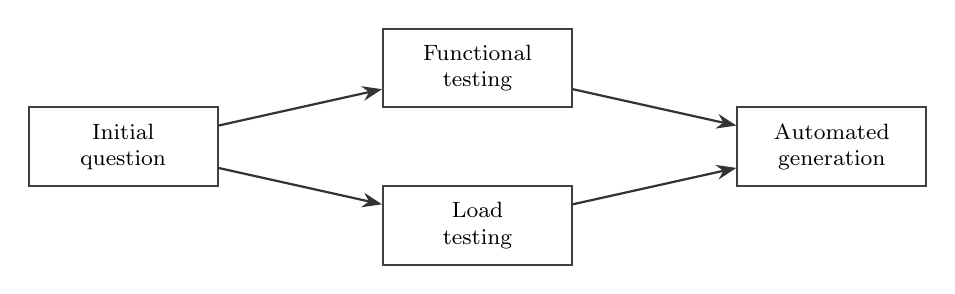
\begin{tikzpicture}[>={Stealth[length=2.5mm]}]
\node[ablock]   (q) at (-5.5,0)    {Initial\\question};
\node[ablock]   (f) at (-1.0, 1.0) {Functional\\testing};
\node[ablock]   (l) at (-1.0,-1.0) {Load\\testing};
\node[ablock]   (a) at ( 3.5,0)    {Automated\\generation};

\draw[aflow] (q) -- node[asig, above, sloped] {} (f);
\draw[aflow] (q) -- node[asig, below, sloped] {} (l);
\draw[aflow] (f) -- (a);
\draw[aflow] (l) -- (a);
\end{tikzpicture}
\end{center}

\vspace{0.8em}
\begin{center}
\textbf{Under what conditions can functional and load testing be \emph{systematically synthesised}\\
from declarative artefacts, rather than authored procedurally per service?}
\end{center}

\vspace{0.4em}
\begin{center}
\footnotesize\itshape
A pre-requisite: the artefacts themselves must be verifiable.
SDT places spec validity inside the framework, not outside it.
\end{center}

\end{frame}

% --------- 3. What we needed -------------------------------------------
\begin{frame}{The artefact at the centre: the specification}

\begin{center}
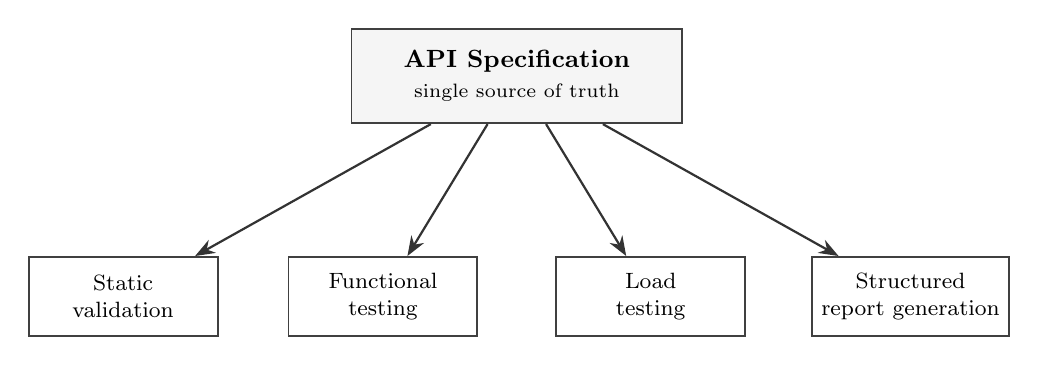
\begin{tikzpicture}[>={Stealth[length=2.5mm]}]
\node[asubject, minimum width=4.2cm, minimum height=1.2cm,
      font=\small\bfseries] (spec) at (0,1.8) {API Specification\\\scriptsize\textnormal{single source of truth}};

\node[ablock] (v) at (-5,  -1) {Static\\validation};
\node[ablock] (f) at (-1.7,-1) {Functional\\testing};
\node[ablock] (l) at ( 1.7,-1) {Load\\testing};
\node[ablock] (r) at ( 5,  -1) {Structured\\report generation};

\draw[aflow] (spec) -- (v);
\draw[aflow] (spec) -- (f);
\draw[aflow] (spec) -- (l);
\draw[aflow] (spec) -- (r);
\end{tikzpicture}
\end{center}

\vspace{0.8em}
\begin{center}
This thesis formalises the resulting paradigm as \alert{\textbf{Specification-Driven Testing (SDT)}}.\\[0.4em]
\footnotesize Each validation task is realised as an orthogonal, composable operation in a unified CLI implementation.
\end{center}

\end{frame}

% --------- 3b. Research questions --------------------------------------
\begin{frame}{Research questions}

\footnotesize
\textbf{RQ1} --- Can automated API quality assurance be operationalised \emph{without dedicated human testers gating the promotion path}, while preserving deterministic and reproducible outcomes?

\vspace{0.6em}
\textbf{RQ2} --- To what extent can the three artefacts of API QA --- \emph{validation rules}
(derived from the OpenAPI \emph{standard}), \emph{executable test cases} (derived from the \emph{specification}),
and \emph{promotion gates} (declared by the tester) --- be mechanically composed into a single
deterministic verification pipeline?

\vspace{0.6em}
\textbf{RQ3} --- How effectively does specification-driven QA compose with cloud-native, GitOps-governed delivery pipelines under continuous reconciliation?

\vspace{0.6em}
\textbf{RQ4} --- Can quality-gated delivery pipelines themselves be expressed as \emph{Kubernetes-native, ontologically structured specifications} --- discoverable, introspectable, and machine-actionable by both operators and autonomous agents?

\vspace{0.8em}
\begin{center}
\alert{Four questions, one unified specification-driven answer.}
\end{center}

\end{frame}

% --------- 3c. Spec drift: the silent problem -------------------------
\begin{frame}{The silent problem: specification--implementation divergence}

\vspace{-0.4em}
\begin{center}
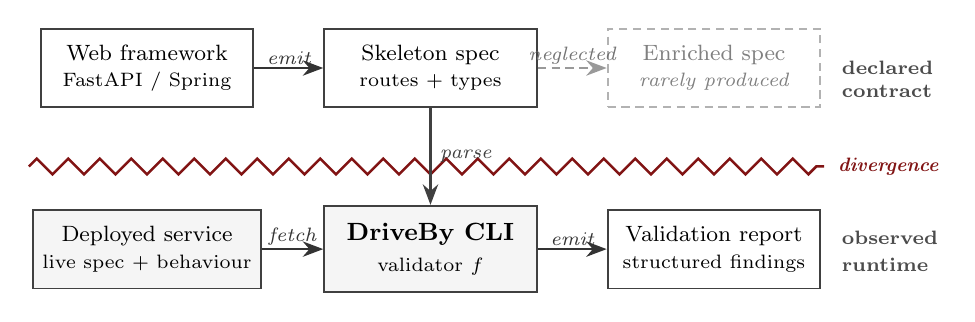
\begin{tikzpicture}[>={Stealth[length=2.6mm]}, font=\small]

% =====================================================================
% Top register: the declared contract (what tooling sees)
% =====================================================================
\node[ablock, minimum width=2.7cm] (fw)
  at (-3.6, 1.7) {Web framework\\\scriptsize FastAPI / Spring};
\node[ablock, minimum width=2.7cm] (skel)
  at ( 0.0, 1.7) {Skeleton spec\\\scriptsize routes $+$ types};
\node[ablock, minimum width=2.7cm, draw=black!30, text=black!50,
      densely dashed]
  (enr)  at ( 3.6, 1.7) {Enriched spec\\\scriptsize \itshape rarely produced};

\node[anchor=west, font=\scriptsize\bfseries, text=black!70]
  at (5.1, 1.7) {declared};
\node[anchor=west, font=\scriptsize\bfseries, text=black!70]
  at (5.1, 1.4) {contract};

\draw[aflow] (fw) -- node[asig, above] {emit} (skel);
\draw[->, line width=0.8pt, black!40, densely dashed]
  (skel) -- node[asig, above, text=black!55, font=\scriptsize\itshape] {neglected} (enr);

% =====================================================================
% Divergence band (red zigzag separating the two registers)
% =====================================================================
\draw[decorate, decoration={zigzag, segment length=4mm, amplitude=1mm},
      line width=0.9pt, sdtred!70!black]
  (-5.1, 0.45) -- (5.0, 0.45);
\node[anchor=west, font=\scriptsize\bfseries\itshape, text=sdtred!70!black,
      fill=white, inner sep=2pt]
  at (5.1, 0.45) {divergence};

% =====================================================================
% Bottom register: observed runtime
% =====================================================================
\node[ablock, minimum width=2.7cm, fill=black!4]
  (live) at (-3.6, -0.6) {Deployed service\\\scriptsize live spec $+$ behaviour};
\node[asubject, minimum width=2.7cm, minimum height=1.1cm,
      font=\small\bfseries]
  (cli)  at ( 0.0, -0.6) {DriveBy CLI\\\scriptsize\textnormal{validator $f$}};
\node[ablock, minimum width=2.7cm]
  (rep)  at ( 3.6, -0.6) {Validation report\\\scriptsize structured findings};

\node[anchor=west, font=\scriptsize\bfseries, text=black!70]
  at (5.1, -0.45) {observed};
\node[anchor=west, font=\scriptsize\bfseries, text=black!70]
  at (5.1, -0.80) {runtime};

\draw[aflow] (live) -- node[asig, above] {fetch} (cli);
\draw[aflow] (cli)  -- node[asig, above] {emit} (rep);

% =====================================================================
% Cross-register validation: spec --> CLI
% =====================================================================
\draw[->, line width=0.8pt, black!75]
  (skel.south) -- node[asig, right=2pt, pos=0.5] {parse} (cli.north);

\end{tikzpicture}
\end{center}

\vspace{-0.4em}
\scriptsize
\begin{itemize}\setlength\itemsep{0.2em}
\item \textbf{\textcolor{sdtred!70!black}{Issue 1.}} Web frameworks emit a
  \emph{structural skeleton} and \alert{none preserves specification--implementation
  parity over time} --- the declared contract drifts away from the deployed service.
\item \textbf{\textcolor{sdtred!70!black}{Issue 2.}} No framework \alert{enriches the
  contract} with semantic descriptors --- example payloads for requests and responses,
  error semantics, operation summaries, security schemes --- that render the spec
  consumable by humans, tooling, and autonomous agents.
\item \textbf{\textcolor{sdtgreen}{Solution: DriveBy.}} The running service is ground
  truth on two fronts --- the \emph{live spec} it publishes (\texttt{/openapi.json},
  checked against the declared spec) and its \emph{live behaviour} (P006/P007).
  \alert{No contradiction with ``spec is the source of truth'':} the declared spec is
  the committed contract; the service is what actually runs; divergence is the finding.
\end{itemize}

\end{frame}

% --------- 4. The DriveBy CLI: parallel principles + aggregation ------
\begin{frame}{DriveBy: the reference implementation}

\vspace{-0.6em}
\begin{center}
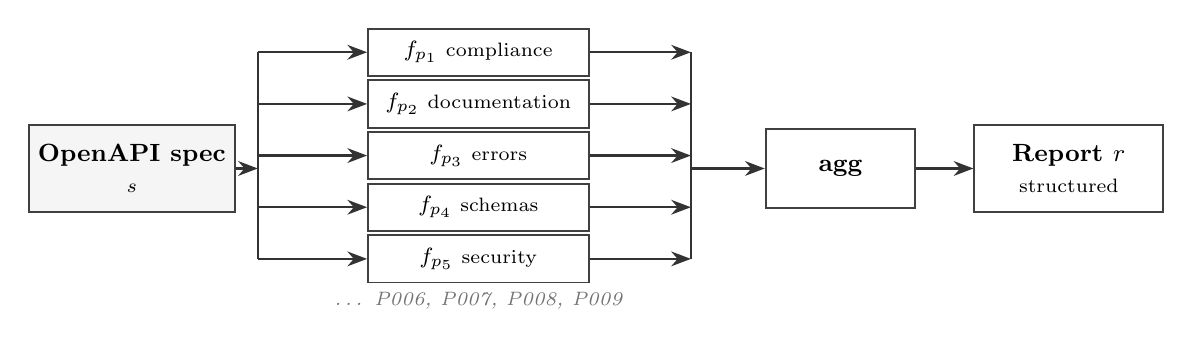
\begin{tikzpicture}[>={Stealth[length=2.5mm]}, font=\small, yscale=0.82]

% Input spec
\node[asubject, minimum width=2.6cm, minimum height=1.1cm,
      font=\small\bfseries] (spec) at (-5.6, 0)
  {OpenAPI spec\\\scriptsize\textnormal{$s$}};

% Fan-out column (invisible coordinate just right of spec)
\coordinate (fanout) at (-4.0, 0);

% Fan-in column (invisible coordinate just left of agg)
\coordinate (fanin) at (1.5, 0);

% Principle functions stacked vertically
\node[ablock, minimum width=2.8cm, minimum height=0.6cm] (p1) at (-1.2,  1.8) {$f_{p_1}$ \scriptsize compliance};
\node[ablock, minimum width=2.8cm, minimum height=0.6cm] (p2) at (-1.2,  1.0) {$f_{p_2}$ \scriptsize documentation};
\node[ablock, minimum width=2.8cm, minimum height=0.6cm] (p3) at (-1.2,  0.2) {$f_{p_3}$ \scriptsize errors};
\node[ablock, minimum width=2.8cm, minimum height=0.6cm] (p4) at (-1.2, -0.6) {$f_{p_4}$ \scriptsize schemas};
\node[ablock, minimum width=2.8cm, minimum height=0.6cm] (p5) at (-1.2, -1.4) {$f_{p_5}$ \scriptsize security};
\node[font=\scriptsize\itshape, text=black!55] at (-1.2, -2.05) {\dots\ P006, P007, P008, P009};

% Aggregation node
\node[ablock, minimum width=1.9cm, minimum height=1.0cm,
      font=\small\bfseries] (agg) at (3.4, 0) {agg};

% Output
\node[ablock, minimum width=2.4cm, minimum height=1.1cm,
      font=\small\bfseries] (rep) at (6.3, 0)
  {Report $r$\\\scriptsize\textnormal{structured}};

% Fan-out: spec -> column -> each principle west
\draw[aflow] (spec.east) -- (fanout);
\draw[line width=0.8pt, black!80] (fanout |- p1) -- (fanout |- p5);
\draw[aflow] (fanout |- p1) -- (p1.west);
\draw[aflow] (fanout |- p2) -- (p2.west);
\draw[aflow] (fanout |- p3) -- (p3.west);
\draw[aflow] (fanout |- p4) -- (p4.west);
\draw[aflow] (fanout |- p5) -- (p5.west);

% Fan-in: each principle east -> column -> agg west
\draw[aflow] (p1.east) -- (fanin |- p1);
\draw[aflow] (p2.east) -- (fanin |- p2);
\draw[aflow] (p3.east) -- (fanin |- p3);
\draw[aflow] (p4.east) -- (fanin |- p4);
\draw[aflow] (p5.east) -- (fanin |- p5);
\draw[line width=0.8pt, black!80] (fanin |- p1) -- (fanin |- p5);
\draw[aflow] (fanin) -- (agg.west);

% Aggregation -> report
\draw[aflow] (agg.east) -- (rep.west);

\end{tikzpicture}
\end{center}

\vspace{-0.4em}
\begin{center}
\small
$f_p(s) \;=\; \mathrm{agg}\bigl(f_{p_1}(s),\, f_{p_2}(s),\, \dots,\, f_{p_n}(s)\bigr)$
\end{center}

\vspace{0.1em}
\footnotesize
\begin{itemize}\setlength\itemsep{0.1em}
\item \emph{Parallel application}, not composition: no $f_{p_i}$ consumes another's output.
\item Each $f_{p_i}$ is atomic, side-effect-free, order-independent --- the
  property that makes Determinism hold and validation modes modular.
\end{itemize}

\end{frame}

% --------- 4b. SDT framework: axioms, principles, validation modes ----
\begin{frame}{The SDT framework: three axioms, nine principles, four modes}

\vspace{-0.3em}
\begin{columns}[T,onlytextwidth]

\column{0.34\textwidth}
\textbf{\textcolor{sdtblue}{Three axioms}}\\[0.15em]
\footnotesize
\begin{itemize}\setlength\itemsep{0.25em}
\item \textbf{Completeness} --- the specification fully describes
  the API contract.
\item \textbf{Determinism} --- identical inputs yield
  identical validation results.
\item \textbf{Observability} --- every validation output is structured,
  quantifiable, machine-readable.
\end{itemize}

\column{0.34\textwidth}
\textbf{\textcolor{sdtblue}{Nine principles}}\\[0.15em]
\scriptsize
\begin{tabular}{@{}ll@{}}
P001 & Compliance \\
P002 & Documentation \\
P003 & Error handling \\
P004 & Schemas \\
P005 & Security \\
P006 & Functional \\
P007 & Performance \\
P008 & Versioning \\
P009 & Test readiness \\
\end{tabular}\\[0.4em]
\tiny Every principle satisfies all three axioms jointly.

\column{0.32\textwidth}
\textbf{\textcolor{sdtblue}{Validation modes}}\\[0.15em]
\scriptsize
\begin{itemize}\setlength\itemsep{0.2em}
\item \textbf{minimal} --- P001 only.\\\textit{fast pre-commit}
\item \textbf{test-ready} --- P001--P004, P009.\\\textit{pre-flight check}
\item \textbf{strict} --- P001--P005, P008.\\\textit{release gate}
\item \textbf{test-only} --- P006, P007.\\\textit{runtime gate}
\end{itemize}

\end{columns}

\vspace{0.6em}
\begin{center}
\footnotesize
\alert{Spec validity is a \emph{first-class output} of the framework, not a pre-condition} ---
P001--P005 probe the spec; P006 probes the live API and detects drift.
\end{center}

\end{frame}

% --------- 5. Reality in industry today --------------------------------
\begin{frame}{Industrial practice vs.\ the SDT proposition}

\begin{columns}[T,onlytextwidth]

\column{0.48\textwidth}
\textbf{\textcolor{sdtred}{Industrial practice}}\\[0.4em]
\footnotesize
\begin{itemize}\setlength\itemsep{0.25em}
\item QA fragmented across siloed actors with no shared protocol.
\item Verification reduced to discretionary, ad-hoc sign-offs.
\item Expert capacity consumed by \emph{repetitive manual procedure} ---
  diverted from process improvement.
\end{itemize}

\column{0.48\textwidth}
\textbf{\textcolor{sdtgreen}{SDT contribution}}\\[0.4em]
\footnotesize
\begin{itemize}\setlength\itemsep{0.25em}
\item Unified framework with structured, machine-actionable artefacts.
\item Each verification step is a deterministic, executable operation.
\item \emph{Orchestration of operations} replaces manual choreography;
  human effort redirected to \emph{methodological and system improvement}.
\item QA promoted to \alert{first-class system component}.
\end{itemize}

\end{columns}

\vspace{0.8em}
\begin{center}
\alert{The bottleneck is not the testing --- it is the manual
choreography that surrounds it.}
\end{center}

\end{frame}

% --------- 6. Cloud-native deployment: declarative composition --------
\begin{frame}{Cloud-native delivery as a Kubernetes-native specification}

\begin{center}
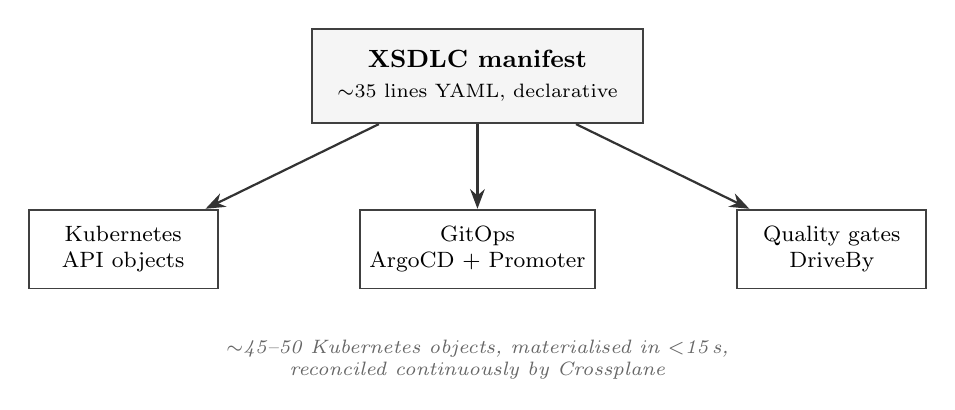
\begin{tikzpicture}[>={Stealth[length=2.5mm]}]
\node[asubject, minimum width=4.2cm, minimum height=1.2cm,
      font=\small\bfseries] (cr) at (0,2.2) {XSDLC manifest\\\scriptsize\textnormal{$\sim$35 lines YAML, declarative}};

\node[ablock] (k8s)    at (-4.5, 0) {Kubernetes\\API objects};
\node[ablock] (gitops) at ( 0,   0) {GitOps\\ArgoCD + Promoter};
\node[ablock] (gates)  at ( 4.5, 0) {Quality gates\\DriveBy};

\draw[aflow] (cr) -- (k8s);
\draw[aflow] (cr) -- (gitops);
\draw[aflow] (cr) -- (gates);

\node[asig, text=black!60, align=center] at (0,-1.4)
  {$\sim$45--50 Kubernetes objects, materialised in $<$15\,s,\\
   reconciled continuously by Crossplane};
\end{tikzpicture}
\end{center}

\vspace{0.2em}
\begin{center}
\footnotesize Identical declarative idiom to the API specification itself ---
\alert{the delivery pipeline is itself a structurally typed,
machine-discoverable specification.}
\end{center}

\end{frame}

% --------- 6b. XSDLC manifest example ---------------------------------
\begin{frame}[fragile]{What an XSDLC manifest actually looks like}

\vspace{0.1em}
\begin{lstlisting}
apiVersion: driveby.io/v1alpha1
kind: XSDLC
metadata: { name: perfect-api }
spec:
  gitopsRepository: { owner: novelcore, name: perfect-api-gitops }
  apiConfig:          { port: 8000, openapiEndpoint: /openapi.json }
  validationDefaults: { validationMode: strict }
  environments:
    - { name: dev }
    - name: staging
      gate: { checks: [ { type: validate-only,
              validationConfig: { validationMode: test-ready } },
              { type: functional-test } ] }
    - name: prod
      autoMerge: false
      gate: { checks: [ { type: load-test, loadTestConfig:
              { concurrentUsers: 10, testDuration: "15s",
                maxLatencyP95: "2s", minSuccessRate: 0.5 } } ] }
\end{lstlisting}

\vspace{0.15em}
\scriptsize
$\sim$35 YAML lines $\to$ $\sim$45--50 Kubernetes objects in $<$15\,s; the
\texttt{Promoter} opens PRs between environment branches and each PR triggers the
declared gate checks before auto-merge.\\[0.2em]
\alert{Check types map to principles:}\quad
\texttt{validate-only} $\to$ P001--P005, P008 \;$\cdot$\;
\texttt{functional-test} $\to$ P006 \;$\cdot$\;
\texttt{load-test} $\to$ P007

\end{frame}

% --------- 7. Consumers of the system ---------------------------------
\begin{frame}{System consumers}

\begin{center}
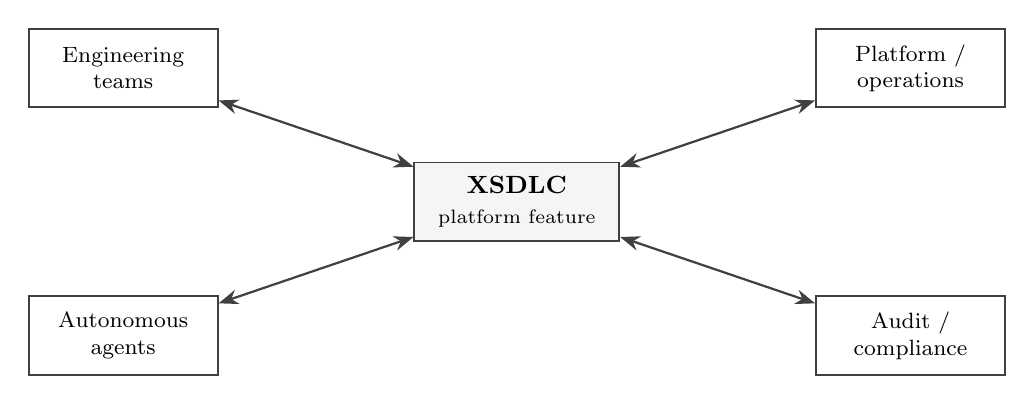
\begin{tikzpicture}[>={Stealth[length=2.5mm]}]
\node[asubject, minimum width=2.6cm, minimum height=1.0cm,
      font=\small\bfseries] (sdt) at (0,0) {XSDLC\\\scriptsize\textnormal{platform feature}};

\node[ablock] (eng)   at (-5.0, 1.7) {Engineering\\teams};
\node[ablock] (ops)   at ( 5.0, 1.7) {Platform /\\operations};
\node[ablock] (agent) at (-5.0,-1.7) {Autonomous\\agents};
\node[ablock] (audit) at ( 5.0,-1.7) {Audit /\\compliance};

\draw[<->, line width=0.8pt, black!75] (sdt) -- (eng);
\draw[<->, line width=0.8pt, black!75] (sdt) -- (ops);
\draw[<->, line width=0.8pt, black!75] (sdt) -- (agent);
\draw[<->, line width=0.8pt, black!75] (sdt) -- (audit);
\end{tikzpicture}
\end{center}

\vspace{0.2em}
\scriptsize
\begin{itemize}\setlength\itemsep{0.15em}
\item \textbf{Engineers} --- declare desired state; XSDLC reifies it.
\item \textbf{Operations} --- interact via standard Kubernetes-native primitives; zero proprietary surface area.
\item \textbf{Autonomous agents} --- consume structured findings as a closed-form, machine-actionable feedback signal.
\item \textbf{Audit \& compliance} --- inherit reproducible, machine-verifiable evidence with intrinsic provenance.
\end{itemize}

\end{frame}

% --------- 7b. End-to-end gate procedure -------------------------------
\begin{frame}{The end-to-end gate procedure}

\vspace{-0.2em}
\begin{center}
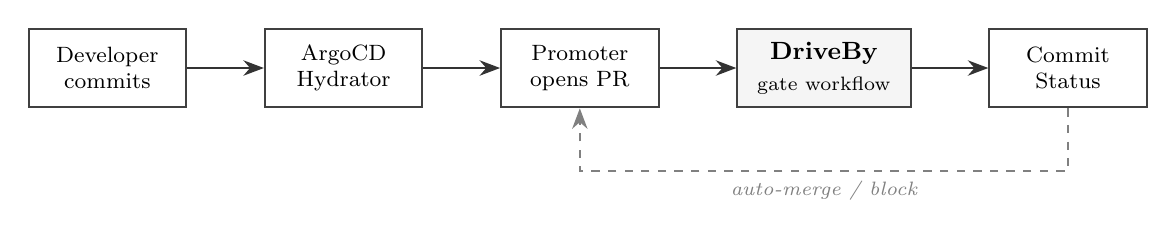
\begin{tikzpicture}[>={Stealth[length=2.6mm]}, font=\small]

\node[ablock, minimum width=2.0cm] (push) at (-6.2, 0) {Developer\\commits};
\node[ablock, minimum width=2.0cm] (hyd)  at (-3.2, 0) {ArgoCD\\Hydrator};
\node[ablock, minimum width=2.0cm] (pr)   at (-0.2, 0) {Promoter\\opens PR};
\node[asubject, minimum width=2.2cm, minimum height=1.0cm, font=\small\bfseries]
     (gate) at ( 2.9, 0) {DriveBy\\\scriptsize\textnormal{gate workflow}};
\node[ablock, minimum width=2.0cm] (cs)   at ( 6.0, 0) {Commit\\Status};

\draw[aflow] (push) -- (hyd);
\draw[aflow] (hyd)  -- (pr);
\draw[aflow] (pr)   -- (gate);
\draw[aflow] (gate) -- (cs);

% Feedback loop: commit status -> PR auto-merge/block
\draw[->, line width=0.8pt, black!50, dashed]
  (cs.south) -- ++(0,-0.8) -| node[asig, near start, below=2pt] {auto-merge / block} (pr.south);

\end{tikzpicture}
\end{center}

\vspace{0.6em}
\footnotesize
\begin{itemize}\setlength\itemsep{0.25em}
\item \textbf{Trigger.} The Promoter opens a PR from \texttt{env-next} to the active environment branch; the gate Workflow fires on PR open.
\item \textbf{Validate.} DriveBy probes the \emph{source} environment (where the new code already runs) and emits a structured report.
\item \textbf{Decide.} The Workflow writes a \texttt{CommitStatus} (\textcolor{sdtgreen!60!black}{pass}: auto-merge $\to$ ArgoCD syncs target; \textcolor{sdtred!70!black}{fail}: PR stays open, developer iterates).
\item \textbf{One declarative trigger; one workflow; one binary decision} --- the entire promotion gate is reified as Kubernetes objects.
\end{itemize}

\end{frame}

% --------- 8a. Control loop: classical block diagram ------------------
\begin{frame}{Closed-loop quality control: classical block diagram}

\vspace{-0.3em}
\begin{center}
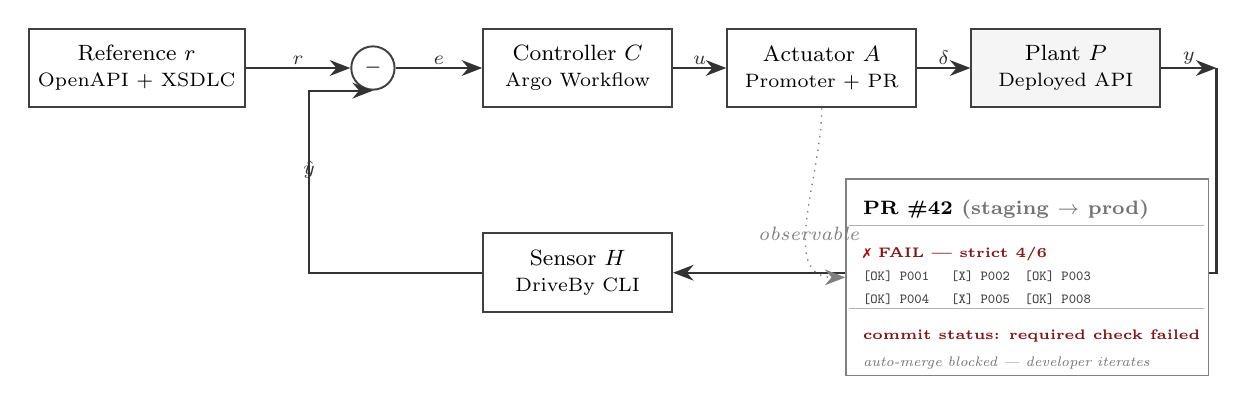
\begin{tikzpicture}[
    >={Stealth[length=2.6mm,width=2mm]},
    font=\small,
    block/.style={rectangle, draw=black!75, fill=white,
                  minimum width=2.4cm, minimum height=1.0cm,
                  align=center, font=\footnotesize, line width=0.7pt},
    plant/.style={rectangle, draw=black!75, fill=black!4,
                  minimum width=2.4cm, minimum height=1.0cm,
                  align=center, font=\footnotesize, line width=0.7pt},
    sumnode/.style={circle, draw=black!75, fill=white,
                    minimum size=0.55cm, inner sep=0pt,
                    font=\scriptsize, line width=0.7pt},
    sig/.style={font=\scriptsize\itshape, inner sep=1pt},
    flow/.style={->, line width=0.8pt, black!80}]

% --- Forward path: r --> sum --> C --> A --> P --> y -------------------
\node[block] (ref)  at (0,    0) {Reference $r$\\\scriptsize OpenAPI $+$ XSDLC};
\node[sumnode] (sum) at (3.0,  0) {};
\node[sig] at (3.0,0) {$-$};
\node[block] (ctrl) at (5.6,  0) {Controller $C$\\\scriptsize Argo Workflow};
\node[block] (act)  at (8.7,  0) {Actuator $A$\\\scriptsize Promoter + PR};
\node[plant] (plant) at (11.8, 0) {Plant $P$\\\scriptsize Deployed API};

\draw[flow] (ref)  -- node[sig, above] {$r$} (sum);
\draw[flow] (sum)  -- node[sig, above] {$e$} (ctrl);
\draw[flow] (ctrl) -- node[sig, above] {$u$} (act);
\draw[flow] (act)  -- node[sig, above] {$\delta$} (plant);

% Output y emerging from plant
\draw[flow] (plant.east) -- ++(0.7,0)
  node[sig, above, pos=0.5] {$y$}
  coordinate (yout);

% --- Feedback path: y -> sensor -> measurement -> sum ------------------
\node[block] (sensor) at (5.6, -2.6) {Sensor $H$\\\scriptsize DriveBy CLI};

\draw[flow] (yout) |- (sensor.east);
\draw[flow] (sensor.west) -- ++(-2.2,0) |- node[sig, above, pos=0.25] {$\hat{y}$} (sum.south);

% --- Visual zoom-in: PR commit-status snapshot (right side, below y) ---
\node[draw=black!50, line width=0.5pt, fill=white,
      minimum width=4.6cm, minimum height=2.5cm,
      anchor=north west] (pr) at (9.0, -1.4) {};

\node[anchor=north west, font=\scriptsize\bfseries]
  at (9.1, -1.55) {PR \#42 \textcolor{black!55}{(staging $\to$ prod)}};
\draw[black!30] (9.05, -2.0) -- (13.55, -2.0);

\node[anchor=north west, font=\tiny\bfseries, text=sdtred!70!black]
  at (9.1, -2.15) {\xmark\ FAIL --- strict 4/6};
\node[anchor=north west, font=\tiny\ttfamily, text=black!75]
  at (9.1, -2.45) {[OK] P001\ \ \ [X] P002\ \ [OK] P003};
\node[anchor=north west, font=\tiny\ttfamily, text=black!75]
  at (9.1, -2.75) {[OK] P004\ \ \ [X] P005\ \ [OK] P008};
\draw[black!30] (9.05, -3.05) -- (13.55, -3.05);
\node[anchor=north west, font=\tiny\bfseries, text=sdtred!70!black]
  at (9.1, -3.20) {commit status: required check failed};
\node[anchor=north west, font=\tiny\itshape, text=black!55]
  at (9.1, -3.55) {auto-merge blocked --- developer iterates};

% Dotted "this is what the actuator emits" arrow from A to PR
\draw[->, line width=0.5pt, black!50, dotted]
  (act.south) to[out=-90,in=180] node[sig, midway, below=2pt] {observable} (pr.west);

\end{tikzpicture}
\end{center}

\vspace{-0.2em}
\begin{center}
\footnotesize
$e(t) = r(t) - H\!\left(y(t)\right)$, \quad $r = (r_{\text{OpenAPI}}, r_{\text{XSDLC}})$. \quad
The promotion gate is the actuator; \emph{the verdict tier is open-loop} ---
the controller decides pass/block, but does not emit a corrective $u$ that reduces $e(t)$.
\end{center}

\vspace{0.05em}
\begin{center}
\tiny\itshape
The promotion chain blocks any production-bound transition that has not first passed P006 ---
drift cannot land in production by construction. Closing the verdict tier (agent-driven
remediation) is the natural continuation --- see Future Work.
\end{center}

\end{frame}

% --------- 8b. Control loop: how the controller is actually realised --
\begin{frame}{How the controller is actually realised: a controller stack}

\vspace{-0.2em}
\begin{center}
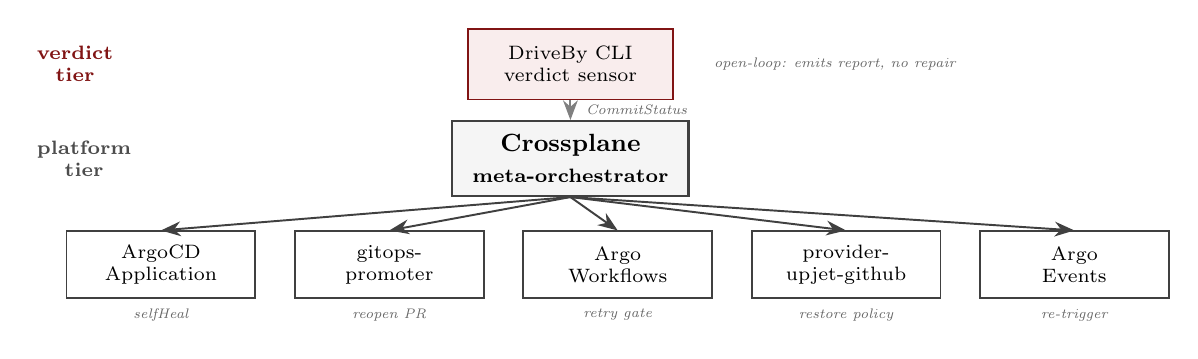
\begin{tikzpicture}[>={Stealth[length=2.5mm]}, font=\small, yscale=0.75,
    tier/.style={rectangle, draw=black!75, fill=white,
                 minimum width=2.4cm, minimum height=0.85cm,
                 align=center, font=\scriptsize, line width=0.7pt},
    meta/.style={rectangle, draw=black!75, fill=black!4,
                 minimum width=3.0cm, minimum height=0.95cm,
                 align=center, font=\small\bfseries, line width=0.8pt},
    verdict/.style={rectangle, draw=sdtred!70!black, fill=sdtred!8,
                    minimum width=2.6cm, minimum height=0.9cm,
                    align=center, font=\scriptsize, line width=0.7pt},
    caplab/.style={font=\tiny\itshape, text=black!60}]

% Verdict tier (top)
\node[verdict] (driveby) at (0, 2.4)
  {DriveBy CLI\\\scriptsize verdict sensor};
\node[caplab, anchor=west] at (1.7, 2.4) {open-loop: emits report, no repair};

% Meta-orchestrator
\node[meta] (cp) at (0, 0.8) {Crossplane\\\scriptsize meta-orchestrator};

% Platform tier (bottom row)
\node[tier] (argo)   at (-5.2, -1.0) {ArgoCD\\\scriptsize Application};
\node[tier] (promo)  at (-2.3, -1.0) {gitops-\\promoter};
\node[tier] (wf)     at ( 0.6, -1.0) {Argo\\Workflows};
\node[tier] (upjet)  at ( 3.5, -1.0) {provider-\\upjet-github};
\node[tier] (events) at ( 6.4, -1.0) {Argo\\Events};

% Crossplane orchestrates each platform controller
\draw[->, line width=0.7pt, black!75] (cp.south) -- (argo.north);
\draw[->, line width=0.7pt, black!75] (cp.south) -- (promo.north);
\draw[->, line width=0.7pt, black!75] (cp.south) -- (wf.north);
\draw[->, line width=0.7pt, black!75] (cp.south) -- (upjet.north);
\draw[->, line width=0.7pt, black!75] (cp.south) -- (events.north);

% DriveBy reads from platform (probe) and writes to gate (CommitStatus)
\draw[->, line width=0.7pt, black!50, dashed]
  (driveby.south) -- node[caplab, right=2pt, pos=0.5] {CommitStatus} (cp.north);

% Repair caption row (under each platform controller)
\node[caplab] at (-5.2, -1.85) {selfHeal};
\node[caplab] at (-2.3, -1.85) {reopen PR};
\node[caplab] at ( 0.6, -1.85) {retry gate};
\node[caplab] at ( 3.5, -1.85) {restore policy};
\node[caplab] at ( 6.4, -1.85) {re-trigger};

% Tier labels
\node[font=\scriptsize\bfseries, text=sdtred!70!black, anchor=west, align=center]
  at (-6.9, 2.4) {verdict\\tier};
\node[font=\scriptsize\bfseries, text=black!70, anchor=west, align=center]
  at (-6.9, 0.8) {platform\\tier};

\end{tikzpicture}
\end{center}

\vspace{0.1em}
\footnotesize
\begin{itemize}\setlength\itemsep{0.15em}
\item Each CRD has its own controller and own reconciliation loop ---
  drift is repaired at the level of the CRD that observes it.
\item \alert{Crossplane} composes $\sim$45--50 managed objects from one XSDLC manifest.
\item The \alert{verdict tier} (DriveBy) is intentionally open-loop ---
  closing it with agent-driven remediation is the natural continuation.
\end{itemize}

\end{frame}

% --------- 9a. Empirical evidence I: systemic quality gap -------------
\begin{frame}{Empirical evidence I: a systemic, cross-vendor quality gap}

\begin{center}
\small
\textbf{APIs.guru, strict policy} ---
\footnotesize 70 providers (50 OpenAPI 3.x $+$ 20 Swagger 2.0)
\end{center}

\vspace{-0.2em}
\begin{center}
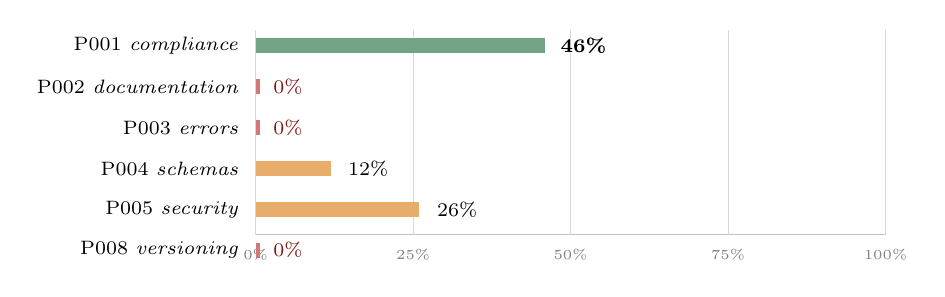
\begin{tikzpicture}[font=\footnotesize, yscale=0.65]

% Axis & gridlines
\draw[gray!50, thin] (0, -1.7) -- (8, -1.7);
\foreach \x/\lbl in {0/0\%, 2/25\%, 4/50\%, 6/75\%, 8/100\%} {
  \draw[gray!30, thin] (\x, -1.7) -- (\x, 2.3);
  \node[font=\tiny, text=gray, anchor=north] at (\x, -1.78) {\lbl};
}

% Bars (width per principle = pass-rate / 100 * 8cm)
\node[anchor=east, font=\scriptsize] at (-0.1, 2.0) {P001 \scriptsize\itshape compliance};
\node[anchor=east, font=\scriptsize] at (-0.1, 1.2) {P002 \scriptsize\itshape documentation};
\node[anchor=east, font=\scriptsize] at (-0.1, 0.4) {P003 \scriptsize\itshape errors};
\node[anchor=east, font=\scriptsize] at (-0.1,-0.4) {P004 \scriptsize\itshape schemas};
\node[anchor=east, font=\scriptsize] at (-0.1,-1.2) {P005 \scriptsize\itshape security};
\node[anchor=east, font=\scriptsize] at (-0.1,-2.0) {P008 \scriptsize\itshape versioning};

\fill[sdtgreen!60]  (0, 1.85) rectangle (3.68, 2.15);
\fill[sdtred!60]    (0, 1.05) rectangle (0.05, 1.35);
\fill[sdtred!60]    (0, 0.25) rectangle (0.05, 0.55);
\fill[sdtorange!60] (0,-0.55) rectangle (0.96,-0.25);
\fill[sdtorange!60] (0,-1.35) rectangle (2.08,-1.05);
\fill[sdtred!60]    (0,-2.15) rectangle (0.05,-1.85);

\node[anchor=west, font=\scriptsize\bfseries] at (3.75, 2.00) {46\%};
\node[anchor=west, font=\scriptsize, text=sdtred!70!black] at (0.10, 1.20) {0\%};
\node[anchor=west, font=\scriptsize, text=sdtred!70!black] at (0.10, 0.40) {0\%};
\node[anchor=west, font=\scriptsize] at (1.05,-0.40) {12\%};
\node[anchor=west, font=\scriptsize] at (2.18,-1.20) {26\%};
\node[anchor=west, font=\scriptsize, text=sdtred!70!black] at (0.10,-2.00) {0\%};

\end{tikzpicture}
\end{center}

\vspace{-0.2em}
\begin{center}
\footnotesize
\alert{\textbf{84\% of providers score $\leq 1/6$ under strict mode.}}
No specimen passes more than 2 of the 6 evaluated principles --- a systemic,
cross-vendor deficiency.
\end{center}

\end{frame}

% --------- 9b. Empirical evidence II: agent-actionable feedback -------
\begin{frame}{Empirical evidence II: the report alone is sufficient agent feedback}

\begin{columns}[c,onlytextwidth]

\column{0.42\textwidth}
\begin{center}
\textbf{Swagger Petstore (baseline)}\\[0.6em]
\footnotesize
\begin{tabular}{ll}
P001 & \cmark \\
P002 & \xmark \\
P003 & \xmark \\
P004 & \xmark \\
P005 & \xmark \\
P008 & \xmark \\
\hline
\textbf{1/6} & \\
\end{tabular}
\end{center}

\column{0.12\textwidth}
\begin{center}
\Large $\longrightarrow$\\[0.4em]
\scriptsize\itshape one\\agent\\iteration
\end{center}

\column{0.42\textwidth}
\begin{center}
\textbf{After agent remediation}\\[0.6em]
\footnotesize
\begin{tabular}{ll}
P001 & \cmark \\
P002 & \cmark \\
P003 & \cmark \\
P004 & \cmark \\
P005 & \xmark \\
P008 & \xmark \\
\hline
\textbf{4/6} & \footnotesize\itshape ($+$300\%) \\
\end{tabular}
\end{center}

\end{columns}

\vspace{0.6em}
\footnotesize
\begin{itemize}\setlength\itemsep{0.2em}
\item Agent inputs: the DriveBy JSON report \emph{and} the OpenAPI spec under repair
  --- \emph{not} the implementation codebase (Petstore is a third-party API). No
  remediation prompt, no exemplar fix.
\item The agent edited the \emph{specification document} to satisfy the failing
  principles; re-validation confirmed 4/6. The report told it \emph{what} was wrong;
  the spec was \emph{where} it fixed it.
\item \alert{SDT's structured output suffices as machine-actionable feedback}
  --- the agent needed no access to source code to close four of six gaps.
\end{itemize}

\end{frame}

% --------- 9. Empirical contribution: the payoff ----------------------
\begin{frame}{Quantified contribution: from days of manual toil to a self-reconciling system}

\begin{columns}[T,onlytextwidth]

\column{0.48\textwidth}
\textbf{\textcolor{sdtred}{Conventional practice}}\\[0.4em]
\footnotesize
\begin{itemize}\setlength\itemsep{0.25em}
\item Multi-day provisioning per service: quality gates, repositories, branches, identities, ingress routes --- each wired by hand.
\item Configuration drift discovered \emph{post-incident}, not pre-emptively.
\item QA reduced to a sequence of human sign-offs --- non-reproducible, non-auditable.
\end{itemize}

\column{0.48\textwidth}
\textbf{\textcolor{sdtgreen}{This thesis (SDT $+$ XSDLC)}}\\[0.4em]
\footnotesize
\begin{itemize}\setlength\itemsep{0.25em}
\item One declarative manifest; full pipeline materialised in $<$15\,s.
\item \alert{Drift detected \emph{and} reconciled} ---
  \textbf{11 of 12} injected drift scenarios converged automatically.
\item Every lifecycle event is \alert{auditable and discoverable} via the Kubernetes API --- machine-readable provenance for every change.
\item QA promoted from human procedure to a \emph{first-class system component}.
\end{itemize}

\end{columns}

\vspace{0.4em}
\begin{center}
\footnotesize
\alert{Days of expert manual effort $\to$ self-reconciled platform delivery,
with full observability and audit traceability.}
\end{center}

\end{frame}

% --------- 9c. Answers to the research questions ----------------------
\begin{frame}{Answers to the research questions}

\footnotesize\vspace{-0.4em}

\textbf{RQ1} --- \emph{\scriptsize Can QA be operationalised without dedicated human testers gating the path?} \quad \alert{\textbf{Yes}}\\
\scriptsize XSDLC declares the gate; Workflow runs DriveBy on every PR; CommitStatus auto-merges
or blocks --- reproducible, human-free at the verdict step.

\vspace{0.3em}
\footnotesize\textbf{RQ2} --- \emph{\scriptsize To what extent are validation rules, test cases, and promotion gates mechanically derived from the spec?} \quad \alert{\textbf{Differentially}}\\
\scriptsize Rules $\leftarrow$ OpenAPI \emph{standard}; tests $\leftarrow$ spec (P006);
gates $\leftarrow$ XSDLC manifest (human-authored, structurally typed and machine-discoverable).

\vspace{0.3em}
\footnotesize\textbf{RQ3} --- \emph{\scriptsize How effectively does SDT compose with GitOps pipelines under continuous reconciliation?} \quad \alert{\textbf{Natively}}\\
\scriptsize One manifest $\to$ $\sim$45--50 reconciled K8s objects in $<$15\,s;
\textbf{11/12} injected drift scenarios converged automatically under Crossplane $+$ ArgoCD.

\vspace{0.3em}
\footnotesize\textbf{RQ4} --- \emph{\scriptsize Can the delivery pipeline itself be an ontologically structured specification?} \quad \alert{\textbf{Yes}}\\
\scriptsize XSDLC reifies the entire pipeline as a Kubernetes CRD --- discoverable,
introspectable, consumed identically by operators and autonomous agents.

\end{frame}

% --------- 9d. Limitations --------------------------------------------
\begin{frame}{Limitations}

\footnotesize

\begin{itemize}\setlength\itemsep{0.25em}
\item \textbf{Verdict tier is open-loop.} The controller decides
  \emph{promote} or \emph{block} but emits no corrective $u$ that
  reduces $e(t)$ --- the report is consumed externally by a developer
  or agent. (Drift between gates is \emph{not} a separate limitation:
  the promotion chain blocks any production-bound transition that has
  not first passed P006.)

\item \textbf{P006/P007 not yet \texttt{PrincipleChecker}-wrapped.}
  Runtime checks live in \texttt{internal/testing/} but are not exposed
  through the uniform principle interface.

\item \textbf{Single delivery cluster.} Evaluation runs against one
  ArgoCD/Crossplane cluster (\texttt{private.novelcore.org}); multi-cluster
  promotion not exercised.

\item \textbf{Single specification format.} OpenAPI 3.x $+$ Swagger 2.0 only;
  AsyncAPI, gRPC, GraphQL out of scope.

\item \textbf{Binary scoring.} Per-principle pass/fail --- no
  risk-weighted or severity-graded composite metric.
\end{itemize}

\end{frame}

% --------- 9e. Future work --------------------------------------------
\begin{frame}{Future work}

\footnotesize

\begin{columns}[T,onlytextwidth]

\column{0.48\textwidth}
\textbf{\textcolor{sdtblue}{Closing the verdict tier}}\\[0.15em]
\begin{itemize}\setlength\itemsep{0.15em}
\item Agent-driven remediation as a true control action ---
  the DriveBy report feeds a coding agent that proposes a spec or
  implementation patch.
\item Adaptive thresholds: gate criteria adjust to observed system
  maturity, not static config.
\item Risk-weighted scoring: binary pass/fail $\to$ severity-aware
  composite metric.
\end{itemize}

\column{0.48\textwidth}
\textbf{\textcolor{sdtblue}{Extending the framework}}\\[0.15em]
\begin{itemize}\setlength\itemsep{0.15em}
\item P006/P007 as first-class \texttt{PrincipleChecker}s.
\item Multi-format adapters: AsyncAPI, gRPC, GraphQL behind \texttt{APISpec}.
\item Multi-cluster promotion --- outer control loops over a fleet.
\item Scheduled prod-environment gate --- CronWorkflow over the same XSDLC
  composition, covering residual out-of-band drift (engineering, not research).
\item Longitudinal agent-feedback study --- slide 16's single iteration
  generalised to multi-agent, multi-pass statistics.
\end{itemize}

\end{columns}

\end{frame}

% --------- 9f. Contribution boundary: own vs agent-assisted -----------
\begin{frame}{Contribution boundary: own intellectual work vs.\ agent-assisted scope}

\footnotesize

\begin{columns}[T,onlytextwidth]

\column{0.49\textwidth}
\textbf{\textcolor{sdtblue}{Own intellectual contribution}}\\[0.15em]
\begin{itemize}\setlength\itemsep{0.15em}
\item \textbf{SDT paradigm} --- axioms, principles, validation modes.
\item \textbf{DriveBy architecture} --- atomic-principle design,
  parallel-application $+$ aggregation formalism.
\item \textbf{XSDLC composition} --- single CRD for the full pipeline;
  two-repo BYOCI boundary.
\item \textbf{Closed-loop framing} of the gate; two-tier controller architecture.
\item \textbf{Evaluation methodology} --- three-arm design, principle
  injection, APIs.guru study, agent-feedback experiment.
\end{itemize}

\column{0.49\textwidth}
\textbf{\textcolor{sdtblue}{Agent-assisted scope}}\\[0.15em]
\begin{itemize}\setlength\itemsep{0.15em}
\item Routine Go boilerplate inside checker implementations
  (interfaces and tests authored by the candidate).
\item LaTeX typesetting and prose-level revisions.
\item Documentation scaffolding (\texttt{CLAUDE.md} files, READMEs).
\item Tooling: batch-validation scripts, harness utilities.
\end{itemize}

\end{columns}

\vspace{0.3em}
\begin{center}
\scriptsize\itshape
Agent assistance is \emph{development methodology}; every architectural and formal
decision was authored, reviewed, and committed by the candidate.
\end{center}

\end{frame}

% --------- 10. Closing -------------------------------------------------
\begin{frame}{Contributions}

\begin{center}
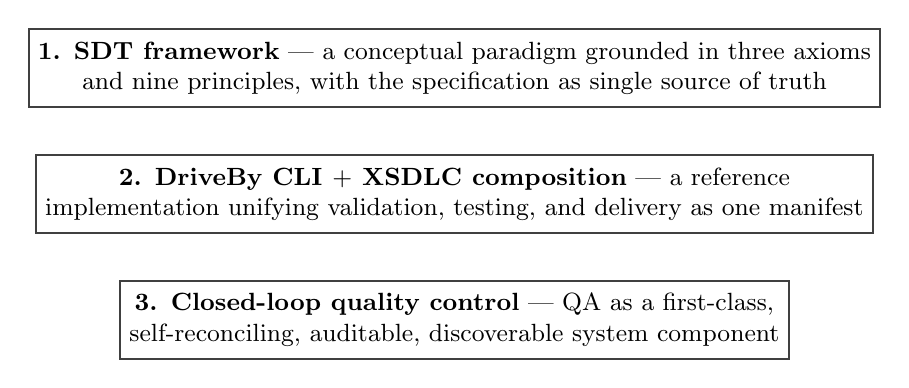
\begin{tikzpicture}
\node[ablock, minimum width=8.5cm, minimum height=1.0cm,
      font=\small] (a) at (0, 1.6)
  {\textbf{1. SDT framework}\ ---\ a conceptual paradigm grounded in three axioms\\
   and nine principles, with the specification as single source of truth};
\node[ablock, minimum width=8.5cm, minimum height=1.0cm,
      font=\small] (b) at (0, 0.0)
  {\textbf{2. DriveBy CLI $+$ XSDLC composition}\ ---\ a reference\\
   implementation unifying validation, testing, and delivery as one manifest};
\node[ablock, minimum width=8.5cm, minimum height=1.0cm,
      font=\small] (c) at (0,-1.6)
  {\textbf{3. Closed-loop quality control}\ ---\ QA as a first-class,\\
   self-reconciling, auditable, discoverable system component};
\end{tikzpicture}
\end{center}

\vspace{0.6em}
\begin{center}
\Large\textbf{Thank you.}\\[0.15em]
\normalsize Questions?
\end{center}

\end{frame}

\end{document}
